\chapter{ارزیابی انطباق}

\section{قسمت اول}

اگر در نمودار زیر، مجموعه نقاط دارای لیبل حقیقی را مجموعه $G=TP \cup FN$ و مجموعه نقاط پیشبینی شده را $M=FP \cup TP$ 
بنامیم؛ آنگاه می‌توان روابط زیر را تعریف کرد.
\begin{center}
\def\firstcircle{(0,0) circle (1.7cm)}
\def\secondcircle{(0:1cm) circle (1.7cm)}

\colorlet{circle edge}{blue!50}
\colorlet{circle area}{blue!20}

\tikzset{filled/.style={fill=circle area, draw=circle edge, thick},
outline/.style={draw=circle edge, thick}}

\setlength{\parskip}{5mm}
% Set A and B
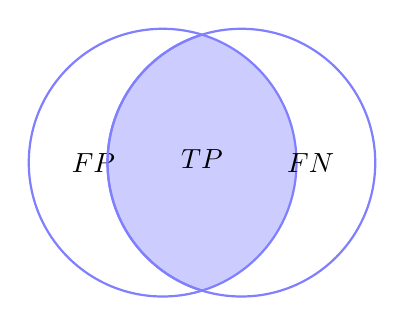
\begin{tikzpicture}
\begin{scope}
	\clip \firstcircle;
	\fill[filled] \secondcircle;
\end{scope}
\draw[outline] \firstcircle node {$FP\qquad\qquad\quad$};
\draw[outline] \secondcircle node {$\qquad\qquad\quad FN$};
\node[anchor=mid] at (current bounding box.base) {$TP$};
\end{tikzpicture}
\end{center}

تعریف معیار \lr{dice}:
\begin{equation}\mathrm{DSC}=\frac{2|M \cap G|}{|M|+|G|} = \frac{2TP}{FP+FN+2TP}\end{equation}

تعریف شاخص \lr{jaccard}:
\begin{equation}\mathrm{JSC}=\frac{|M \cap G|}{|M \cup G|}=\frac{\mathrm{DSC}}{2-\mathrm{DSC}} \end{equation}


تعریف فاصله ی \lr{Hausdorff}:
\begin{equation}\mathrm{HD}=\max \left\{\max _{x \in \partial G} \mathbf{d}(x, \partial M), \max _{y \in \partial M} \mathbf{d}(y, \partial G)\right\}\end{equation}

تعریف فاصله ی \lr{Average symmetric surface}:
\begin{equation}\operatorname{ASSD}=\frac{\sum_{x \in \partial G} \mathbf{d}(x, \partial M)+\sum_{y \in \partial M} \mathbf{d}(y, \partial G)}{|\partial G|+|\partial M|}\end{equation}


برای مطالعه معیار های بیشتر می‌توان به \cite{Zhou2019} مراجعه کرد.

\section{قسمت دوم}

در این قسمت میخواهیم توابعی را بنویسیم که معیار های معرفی شده در قسمت اول را پیاده سازی کنیم. برای این کار ابتدا اطلس و شیفت یافته خودش را باهم دیگر مقایسه کردیم و یکی از آن ها را بعنوان لیبل های واقعی و دیگری را به عنوان لیبل های پیشبینی شده در نظر گرفته شده اند. نتیجه این‌کار که در شکل \ref{fig:partB:pcshowpair-indices}
مشخص شده است، با استفاده از کد زیر آن شیفت ایجاد شده است.


\begin{figure}[t!]
	\centering
	\includegraphics[width=0.7\linewidth]{partB-pcshowpair-indices}
	\vspace{-1em}
	\caption{}
	\label{fig:partB:pcshowpair-indices}
\end{figure}

\begin{latin}
\begin{lstlisting}[frame=none]
atlas = readData('atlas', true);
img3d_true = atlas;
img3d_pred = circshift(atlas, 5);
\end{lstlisting}
\end{latin}

برای مشاهده خروجی های آورده شده در شکل \ref{fig:partB:pcshowpair-indices}
باید فایل \Seemycode{partB.m}
را اجرا کرد. برای این کار توابعی طراحی شده است که در جدول \ref{table:partB:intro-indices}
توضیح داده شده است.

\begin{table}[b!]
	\begin{tabularx}{\textwidth}{|C{0.2\linewidth}| C{0.3\linewidth} | Y |}
		\hline\rowcolor{headerColor} نام معیار & نام تابع & توضیحات \\\hline
		\lr{Hausdorff Distance} & \Seemycode{HausdorffDist.m} & \\\hline		
		\lr{Average Surface Distance} & \Seemycode{AverageSurfaceDist.m} & \\\hline		
		\lr{Binary Dice score} & \Seemycode{binary\_dice\_loss.m} & \\\hline		
		\lr{Dice score} & \Seemycode{dice\_loss.m} & \\\hline		
		\lr{Binary Jaccard Index} & \Seemycode{binary\_jaccard\_loss.m} & \\\hline		
		\lr{Jaccard Index} & \Seemycode{jaccard\_loss.m} & \\\hline		
	\end{tabularx}
	\caption{}
	\label{table:partB:intro-indices}
\end{table}


همچنین برای ایجاد شکلی واحد در صدازدن توابع داده شده، تابع \Seemycode{calc\_loss.m}
طراحی شده است که مثلا برای محاسبه فاصله ی \lr{ASSD} توضیح داده شده در قسمت اول، از تابع زیر استفاده می‌توان کرد و  برای باقی معیار ها نیز کافیست که \verb|@AverageSurfaceDist| را با نام تابع مرتبط در آن معیار که در جدول \ref{table:partB:intro-indices} معرفی شده است، استفاده کرد.


\begin{latin}
\begin{lstlisting}[frame=none]
ASSD = calc_loss(@AverageSurfaceDist,    ptCloud_true, ptCloud_pred);
\end{lstlisting}
\end{latin}


اگر انطباق به طور کامل اتفاق افتاده باشد فاصله های \lr{Hausdorff Distance} و \lr{Average Surface Distance} باید صفر شود و باقی شاخص ها باید یک شود و آن دو فاصله با افزایش مقدار شیفت باید زیاد و باقی معیار ها باید کاهش پیدا کنند. برای تشخیص درستی این مورد، به ازای شیفت های متفاوت این مقادیر محاسبه شده و در جدول \ref{table:varing-shift-indices}
وارد شده است. همانگونه که مشخص است، این توابع توانسته اند این گونه انتظارات بدیهی ما را پاسخ دهند.
%\begin{figure}[t!]
%	\centering
%	\includegraphics[width=0.7\linewidth]{partB-HausdorffDist}
%	\caption{}
%	\label{fig:partB:HausdorffDist}
%\end{figure}


\begin{table}[b!]
	\centering
	\begin{LTR}
		\readcsv{centercolorheader}{../Code/results/partB-table-indices1.csv}
		\readcsv{centercolorheader}{../Code/results/partB-table-indices2.csv}	
	\end{LTR}
	\caption{}
	\label{table:varing-shift-indices}
\end{table}



\begin{note}
	جدول \ref{table:varing-shift-indices} توسط خروجی های کد متلب \Seemycode{partB.m} به صورت کاملا اتوماتیک ایجاد شده است. در حقیقت کد مذکور داده های این جدول را در \Seemycode{results/partB-table-indices1.csv} و \Seemycode{results/partB-table-indices2.csv} ذخیره می‌کند و توسط پکیج \texttt{csvsimple} لاتک در این فایل \lr{pdf} قرار داده شده است.
\end{note}

